\section{Bevezetés}

A dokumentum abból a célból jött létre, hogy segítséget nyújtson \verb!STM32F4-Discovery! board alapú projektek fejlesztéséhez. A szükséges lépések nagyrészét igyekszünk bemutatni valós alkalmazások segítségével, melyeknek túlnyomó többsége a 2014-es \textbf{RobonAUT} versenyre történő felkészülés közben került kivitelezésre. A problémák számunkra is újak voltak, így nem ígérhetjük, hogy a legjobb megoldásokat fogjuk prezentálni itt, de a bemutatott eljárásról kijelenthetjük, hogy hasznosnak és megbízhatónak bizonyult.

Az írást három fő részre osztottuk, először bemutatásra kerülnek a \verb!MATLAB-Simulink! modell alapú tervezés lépései és a fordítható kód generálása. Ezután a generált kód integrálására és élesztésére térünk rá \verb!FreeRTOS! operációs rendszer alatt, legvégül pedig valós gyors prototípustervezési technikák kerülnek bemutatásra, a \verb!MATLAB! közvetlen \verb!STM32F4-Discovery! hardware támogatását felhasználva.

\begin{figure}[!ht]
    \centering
    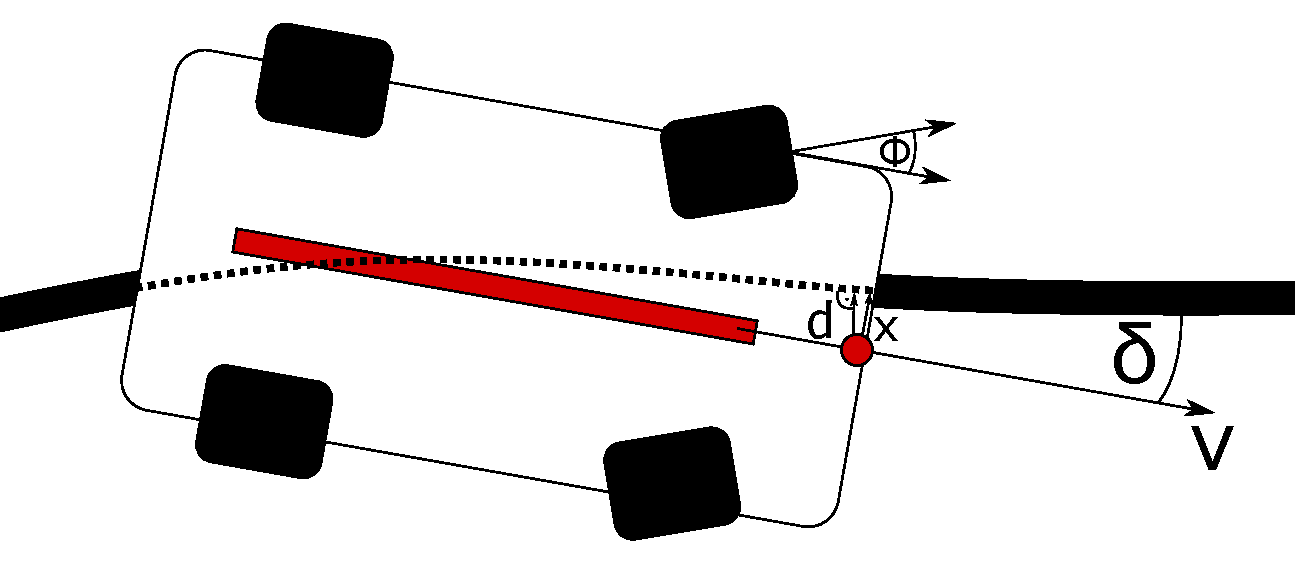
\includegraphics[width=0.9\linewidth]{img/cartop}
    \caption{A probléma sematikus ábrája felülnézetből}
    \label{fig:cartop}
\end{figure}

A \textbf{RobonAUT} verseny során egy olyan robot szoftverét és hardverét kell elkészíteni, amely lehetővé teszi a távirányítós autóból átalakított platformot, hogy egy ismeretlen pályán végighaladjon, és ott akadályokat teljesítsen, a szabályzatban meghatározott módon. A továbbiakban csak a szoftver környezettel foglalkozunk és feltételezzük, hogy megfelelő logikai jelek zajjal terhelten bár, de rendelkezésre állnak a szenzorokból, illetve az autó várakozásainknak megfelelően reagál a kimeneti jelekre, pl. a kormányszög beállítására.

A dokumentumban próbáljuk a szakirodalomban elterjedt jelrendszert alkalmazni, de az alábbi táblázat segítségével magyarázzuk a rendszeresen előforduló jelöléseket és összefüggéseket. Amennyiben valami hiányzik innen, az a szövegkörnyezetben kerül definiálásra.

\begin{center}
  \begin{tabular}{| c | p{0.8\linewidth} |}
\hline
    d & Pozícióhiba: Az első optikai szenzorsor középpontjának távolsága a vonaltól \\ \hline
    $ \delta $ & Szöghiba: Az első optikai szenzorsorra merőleges egyenes (középvonal) és a pályavonal érintője által bezárt szög \\ \hline
    $ \Phi $ & Kormányszög: A kerekek síkjainak a középvonallal bezárt szögeinek átlaga, Ackermann-kormányzás szerint \\
    \hline
    $ \kappa $ & A pálya pillanatnyi görbülete ($1/R$) \\ \hline
    x & Vonalpozíció: az első optikai szenzorsor által érzékelt vonalak középpontjának előjeles távolsága a szenzorsoron a közepponttól mérve. \\ \hline
    c & Vonalsebesség: x első deriváltja, a vonalpozíció mozgásának sebessége \\ \hline
    v & Sebesség: Az autó pillanatnyi sebessége a középvonal mentén \\
    \hline
  \end{tabular}
\end{center}